\section{Secțiunea de mesaje din cadrul cererilor de despăgubire}

	În caz de probleme sau nelămuriri, în cadrul link-ului primit pe mail, o dată ce se navighează la pagina respectivă, se poate apăsa butonul „Messages” pentru a trimite într-un dialog mesaje de la client la utilizator, cum se poate observa în figurile~\ref{fig:message_mail_from_person},~\ref{fig:message_mail_from_office},~\ref{fig:claim_mesaje}.

	De asemenea, același sistem poate fi folosit și de utilizator, pentru a trimite un mesaj clientului, fiecare fiind anunțat pe mail în cazul unui nou mesaj.

	\begin{figure}
		\centering
		\subfigure[Email trimis când clientul trimite un mesaj]{
			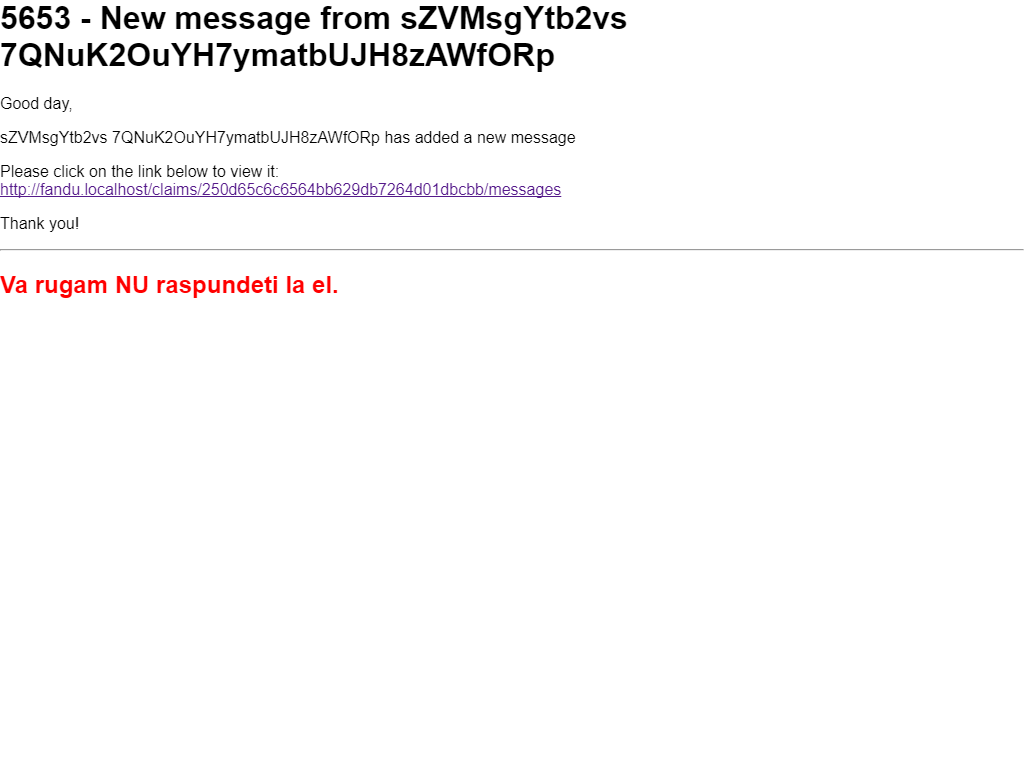
\includegraphics[width=0.4\linewidth, height=0.4\textheight, keepaspectratio]{../imagini/message_mail_from_person.png}
			\label{fig:message_mail_from_person}
		}
		\subfigure[Email trimis când utilizatorul trimite un mesaj]{
			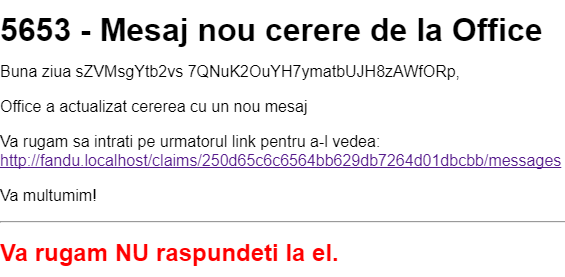
\includegraphics[width=0.4\linewidth, height=0.4\textheight, keepaspectratio]{../imagini/message_mail_from_office.png}
			\label{fig:message_mail_from_office}
		} \\
		\subfigure[Interfața de messages, împreună cu istoricul mesajelor]{
			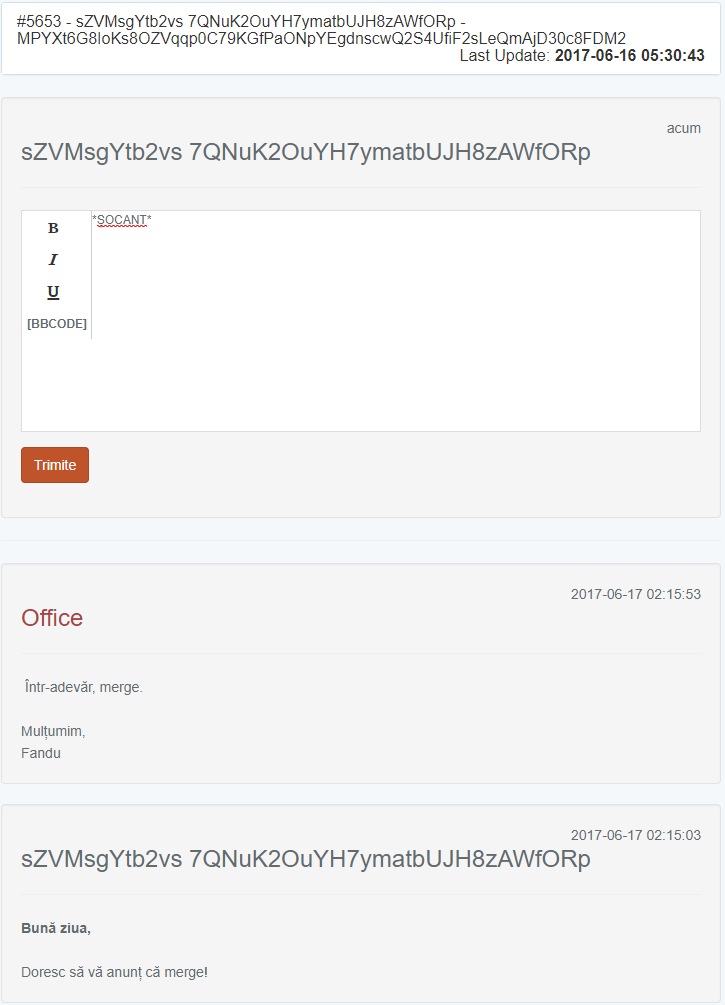
\includegraphics[height=0.6\textheight, keepaspectratio]{../imagini/claim_mesaje.png}
			\label{fig:claim_mesaje}
		}
		\caption{Interacțiunea mesajelor de mesaje}
	\end{figure}
